\documentclass[english,11pt,letterpaper,onecolumn]{scrartcl}

%\usepackage[utf8]{inputenc}
\usepackage{babel}
\usepackage{csquotes}
\usepackage{amsmath}
\usepackage{amsfonts}
\usepackage{mathptmx}
\usepackage{enumitem}
% Extra leading.
\renewcommand{\baselinestretch}{1.125}
\usepackage{tocloft}
% \usepackage{fancyhdr}
\usepackage{scrlayer-scrpage}
\usepackage{ifthen}
\usepackage{keyval}
\usepackage{geometry}
\usepackage{url}
\usepackage{calc}
\usepackage{array}
\usepackage{graphicx}
\usepackage{color}
\usepackage{listings}
\usepackage{supertabular}
% definitions used by included articles, reproduced here for
% educational benefit, and to minimize alterations needed to be made
% in developing this sample file.
\usepackage{amssymb}
\usepackage{latexsym}
\usepackage{amsfonts}
\usepackage{amsmath}
\usepackage{amscd}     % commutative diagrams
\usepackage{mathrsfs}  % This package allows the use of script letters. Type \mathscr to invoke math script.
\usepackage{amsbsy}
%\usepackage{scrpage2}
\usepackage[pdftex,
colorlinks=true,
linkcolor=blue,
pdfpagelabels,
pdfstartpage=3
]{hyperref}
% \usepackage{poemscol}
% \global\verselinenumbersfalse
\makeindex
\definecolor{LstColor}{cmyk}{0.1,0.1,0,0.025}
\setcounter{tocdepth}{9}
\newcommand\floor[1]{\lfloor#1\rfloor}
\newcommand\ceil[1]{\lceil#1\rceil}
\usepackage{lmodern}
\usepackage{amssymb,amsmath}
\usepackage{ifxetex,ifluatex}
\hypersetup{breaklinks=true,
bookmarks=true,
pdfauthor={},
pdftitle={},
colorlinks=true,
citecolor=blue,
urlcolor=blue,
linkcolor=magenta,
pdfborder={0 0 0}}

\usepackage{amsfonts}
\usepackage{amsmath}
\usepackage{amssymb}
\usepackage{graphicx}

\usepackage{version}%
\setcounter{MaxMatrixCols}{30}

%%%% Packages added - Peter
\usepackage{color}
\usepackage{amscd}     % commutative diagrams
\usepackage{mathrsfs}  % This package allows the use of script letters.
%%%%%%%%%%%%%%%%%%%%%%%%%%%%%%%%%%%%%%%%%%%%%%%%%%%%%

\newtheorem{theorem}{Theorem}[section]
%\theoremstyle{plain}
\newtheorem{acknowledgement}{Acknowledgement}
\newtheorem{algorithm}{Algorithm}[section]
\newtheorem{axiom}{Axiom}[section]
\newtheorem{case}{Case}[section]
\newtheorem{claim}{Claim}[section]
\newtheorem{conclusion}{Conclusion}[section]
\newtheorem{condition}{Condition}[section]
\newtheorem{conjecture}{Conjecture}[section]
\newtheorem{corollary}{Corollary}[section]
\newtheorem{criterion}{Criterion}[section]
\newtheorem{definition}{Definition}[section]
\newtheorem{example}{Example}[section]
\newtheorem{exercise}{Exercise}[section]
\newtheorem{lemma}{Lemma}[section]
\newtheorem{notation}{Notation}[section]
\newtheorem{problem}{Problem}[section]
\newtheorem{proposition}{Proposition}[section]
\newtheorem{remark}{Remark}[section]
\newtheorem{solution}{Solution}[section]
\newtheorem{summary}{Summary}[section]
\numberwithin{equation}{section}
\excludeversion{comment1}

%%%%% Macros added - Peter
\newcommand{\st}{\,|\,}
\newcommand{\C}{\mathbb{C}}
\newcommand{\F}{\mathbb{F}}
\newcommand{\I}{\mathbb{I}}
\newcommand{\bH}{\mathbb{H}}
\newcommand{\K}{\mathbb{K}}
\newcommand{\N}{\mathbb{N}}
\newcommand{\Q}{\mathbb{Q}}
\newcommand{\R}{\mathbb{R}}
\newcommand{\T}{\mathbb{T}}
\newcommand{\X}{\mathbb{X}}
\newcommand{\Y}{\mathbb{Y}}
\newcommand{\Z}{\mathbb{Z}}
%
\newcommand{\cB}{\mathcal{B}}
\newcommand{\cC}{\mathcal{C}}
\newcommand{\mcD}{\mathcal{D}}
\newcommand{\cE}{\mathcal{E}}
\newcommand{\cF}{\mathcal{F}}
\newcommand{\cG}{\mathcal{G}}
\newcommand{\calH}{\mathcal{H}}
\newcommand{\cJ}{\mathcal{J}}
\newcommand{\cK}{\mathcal{K}}
\newcommand{\mcL}{\mathcal{L}}
\newcommand{\cM}{\mathcal{M}}
\newcommand{\cN}{\mathcal{N}}
\newcommand{\cO}{\mathcal{O}}
\newcommand{\calR}{\mathcal{R}}
\newcommand{\cS}{\mathcal{S}}
\newcommand{\mcT}{\mathcal{T}}
\newcommand{\cU}{\mathcal{U}}
\newcommand{\cW}{\mathcal{W}}
\newcommand{\cY}{\mathcal{Y}}
\newcommand{\bcF}{\boldsymbol{\mathcal{F}}}
%
\newcommand{\oY}{\overline{Y}}
\newcommand{\uY}{\underline{Y}}
%
\renewcommand{\Re}{\mathop{\mathrm{Re}}}
\renewcommand{\Im}{\mathop{\mathrm{Im}}}
%
\newcommand{\card}{\mathop{\mathrm{card}}}
\newcommand{\Int}{\mathop{\mathrm{int}}}
\newcommand{\eps}{\varepsilon}
\newcommand{\kap}{\varkappa}
\newcommand{\be}{\begin{equation}}
\newcommand{\ee}{\end{equation}}
\newcommand{\inn}[2]{{\langle #1,#2 \rangle}}
\newcommand{\wt}[1]{{\widetilde{#1}}}

\newcommand{\conv}{\mathrm{conv}\,}
\newcommand{\bx}{{\boldsymbol{x}}}
\newcommand{\by}{{\boldsymbol{y}}}
\newcommand{\bk}{{\boldsymbol{k}}}
\newcommand{\bm}{{\boldsymbol{m}}}
\newcommand{\bc}{{\boldsymbol{c}}}
\newcommand{\ba}{{\boldsymbol{a}}}
\newcommand{\bp}{{\boldsymbol{p}}}
\newcommand{\bP}{{\mathbb{P}}}
\newcommand{\bS}{{\boldsymbol{S}}}
\newcommand{\bq}{{\boldsymbol{q}}}
\newcommand{\bfe}{{\boldsymbol{e}}}
\newcommand{\bone}{{\boldsymbol{1}}}
\newcommand{\bu}{{\boldsymbol{u}}}
\newcommand{\bv}{{\boldsymbol{v}}}
\newcommand{\bw}{{\boldsymbol{w}}}
\newcommand{\bff}{{\boldsymbol{f}}}
\newcommand{\bkk}{{\boldsymbol{k-1}}}
\newcommand{\bxi}{{\boldsymbol{Xi}}}
\newcommand{\balpha}{{\boldsymbol{\alpha}}}
\newcommand{\bbeta}{{\boldsymbol{\beta}}}
\newcommand{\bgamma}{{\boldsymbol{\gamma}}}
\newcommand{\blambda}{{\boldsymbol{\lambda}}}
\newcommand{\bmu}{{\boldsymbol{\mu}}}
\newcommand{\gr}{{\mathrm{graph\,}}}
\newcommand{\of}{\overline{f}}
\newcommand{\og}{\overline{g}}
\newcommand{\oc}{\overline{c}}
\newcommand{\ou}{\overline{u}}
\newcommand{\ox}{\overline{x}}
\newcommand{\oX}{\overline{X}}
\newcommand{\oXi}{\overline{X}_i}
\newcommand{\uc}{\underline{c}}
\newcommand{\oy}{\overline{y}}
\newcommand{\uy}{\underline{y}}
\newcommand{\odelta}{\overline{\delta}}
\newcommand{\udelta}{\underline{\delta}}
\newcommand{\oPhi}{\overline{\Phi}}
\newcommand{\map}{\textrm{Map}\,}
\newcommand{\loc}{\mathrm{loc}}
\newcommand{\mydot}{\;\cdot\;}
\DeclareMathOperator{\dom}{dom}
\DeclareMathOperator{\range}{range}
\DeclareMathOperator{\id}{id}
\DeclareMathOperator{\Aff}{Aff}
\DeclareMathOperator{\GL}{GL}
\DeclareMathOperator{\diag}{diag}

\usepackage[
backend=biber,
style=numeric,
sorting=ynt,
hyperref=true,
backref=true
]{biblatex}
\addbibresource{gogins.bib}
\begin{document}

\title{Parametric Composition of Score Graphs}
\author{Michael Gogins \\ \texttt{michael.gogins@gmail.com}}
\maketitle
%\pagestyle{scrheadings}

\begin{abstract}
I present several new related methods for the parametric composition of musical
scores. A scores is defined as the graph of a function of time in chord spaces.
Such graphs are computed using special iterated function systems (IFS) related
to the Read-Bajraktarevi\'c operator. The Collage Theorem proves that any such
graph may be approximated, as closely as desired, by such an IFS. One method of
composing is then to manually construct these IFSs, or to evolve them using the
genetic algorithm, and then to render the IFS to an actual score. Additionally,
using Hilbert indexes, a single complex virtual parameter can be derived to
represent each set (potentially dozens or more numbers) of the IFS parameters
used to compute each score graph. Each virtual parameter may be mapped to the
score produced from the corresponding IFS, thus producing a parametric map of
scores colored by some musical feature of interest. Other methods of composition
are to interactively explore this parametric map, or to interpolate between
different scores located in this map.
\end{abstract}

%\lohead{Parametric Composition}

\section{Introduction}

We define a \textit{score space} as a space in which a set of points represents
a piece of music, \textit{e.g.}\ notes on the grand staff, punches in a piano
roll, some more abstract space, or even grains of sound on a sonogram. We
define a \textit{score generator} as a computer program that generates a
musical score in some score space. We define a \textit{parametric score
generator} as one whose behavior is completely defined by numerical parameters.

Then \textit{parametric composition} is the art of composing music by exploring
the parameter space of some parametric score generator. Such exploration can be
performed by literally zooming around in a colored map of the parameter space,
by interpolating between two parameter points in that space, or by evolving
parameters using the genetic algorithm.

Parametric composition has previously been investigated with respect to the
generation of pieces in spaces that directly represent either sound,
\textit{e.g.}\ in the form of a grid of sound grains (Gabor transform)
\cite{obsessed}, or scores, \textit{e.g.}\ in the form of a grid of notes
(piano roll) \cite{ifsmusic}.

Here, pieces are generated in a score space constructed from time and the basic
symmetries of chord space identified by Callender, Quinn and Tymoczko
\cite{callender:346}, along with revoicings and rearrangements. The dimensions
of this score space are: set class (the most basic form of a  chord) $P$
(\textit{i.e.}, Callender \textit{et al.}'s $OPTIC$), inversion $I$,
transposition $T$, octavewise revoicings $v$, and rearrangements of voices $a$.
In $PITva$ space, a piece of note-based music may be considered a succession of
more or less fleeting chord points or, in other words, as the graph of a
vector-valued function of time in the score space, which we call a
\textit{score graph} of a \textit{score function},

$$(P, I, T, v, a) = r(t).$$

\noindent The notes and chords do \textit{not} need to be confined to 12-tone
equal temperament. One motivation for using score functions to compose is that,
at any one point in time, there is one and only one ``harmony.''

The score generators used here are \textit{iterated function systems} (IFSs)
\cite{barnsley1985iterated, 10.2307/24893080, fractalseverywhere}. More
particularly, our score generators are special IFSs where the contractive
transformations that make up the IFS are constrained such that the IFS computes
not any old attractors, but only attractors that closely approximate the graphs
of functions. These are called \textit{fractal approximations} (FAs) or fractal
interpolations \cite{Barnsley1986, fractalseverywhere, navascues2014fractal}.
The function for such a graph is called simply a \textit{fractal function}. (It
is interesting that all continuous functions are fractal functions
\cite{2016arXiv161001369B}.) Even more particularly, we use FAs to compute
graphs of $r$. The advantage of such FAs is that (in principle) \textit{any}
score can be so generated, and \textit{every} FA of this type generates a graph
of some $r$.

A FA may be completely specified as a set of numerical parameters. Thus, any
piece of note-based music may be approximated as closely as desired by a fixed
size set of numerical parameters.

Although there might be dozens or hundreds of numbers in such FA parameters,
each parameter set can effectively be represented as a single real or complex
number by using a recursive indexing scheme such as a Hilbert index
\cite{hamilton2006compact}. We call this number the \textit{effective parameter}
of the FA because the complete set of parameters can be recovered (given
sufficient numerical precision) by decoding the index.

Then, using the effective parameters, it is simple to compute a parametric map
of all pieces within a given range of FAs, or to interpolate between two pieces
by interpolating between their effective parameters. It is also, of course,
possible to evolve pieces using the genetic algorithm on sets of actual
parameters.

The remainder of this paper develops the mathematical background in somewhat
more detail; discusses the implementation of fractels, fractal approximations,
Hilbert indices, and the genetic algorithm for FA parameters in the Silencio
library for algorithmic composition in JavaScript; and finishes with examples of
each of the three methods of algorithmic composition, implemented in Silencio
and Csound.

\section{Mathematical Development}

This section is not intended as a complete, self-contained exposition but rather
as providing entry points for readers who have some exposure to mathematical
music theory or fractal geometry. I have tried to supply references not only to
original publications of ideas, but also to recent reviews or summaries.

TO DO: Really understand (a) how exactly can the local IFS dual to a RB operator
be implemented in code, and (b) what exactly is a fractal in this context. What
\textit{\textbf{is}} clear is that they are trying specifically to produce IFSs
whose attractors are graphs of functions.

It has become clear that "bilinear transformation" is a bit more general than
"affine transformation." Basically, in this context, a bilinear transformation
is similar to a shear transformation, but the two sides of the image can have
different sizes. It's also clear that the concept originated in 2-dimensional
graphics but can be generalized to N dimensions. Barnsley does give formulas for
deriving the coefficients.

An RB operator is a kind of IFS in which the graph of a function over a segment
$[a, b]$ is approximated by mapping the $[a, b]$ to each of the sub-segments
defined by a pair of interpolation points. For a somewhat more concrete
presentation in the form of a Mathematica workbook, see \cite{McClure2006}.

A \textit{local} IFS is one in which each function or mapping in the IFS may
have a different co-domain, but the domains do not overlap.

Various maps can be used to construct an RB operator for a given graph. Here, we
use local iterated functions instead of plain linear mappings for each
interpolation segment.

\subsection{Chord Spaces}

A \textit{chord space} is simply a space in which each voice of a chord is
represented by a different dimension. A single voice is represented by a point
on a line; an interval, by a point on a plane; a triad, by a point in a
3-dimensional space; and so on. Here the octave is always 12, so that
pitch-classes in 12 TET are always integers (and compatible with MIDI). Chord
space has many uses. For example, Tymoczko \cite{tymoczko2006geometry,
tymoczko2011geometry} showed that perceptually smoother voice-leadings between
chords are represented by shorter distances in chord space.

Even unschooled musicians are aware that pitches transposed to different octaves
are somehow the same. This is expressed in music theory by saying that
pitch-classes, \textit{e.g.} C or F\#, are pitches under \textit{octave
equivalence}. Octave equivalence transforms the line of pitch into a circle, an
\textit{orbifold} or \textit{quotient space} $\mathbb{R}/12$, by gluing the
lowest pitch under octave equivalence to the same pitch an octave higher. There
are other implicitly familiar equivalence classes in music:
\textit{permutational equivalence} (a triad is somehow the same whether the
voices are assigned to violin, trumpet, and flute or to flute, trumpet, and
violin), \textit{cardinality equivalence} (a chord is somehow the same if voices
are doubled in different octaves), and so on. Callender, Quinn, and Tymoczko
\cite{callender:346} have concisely analyzed these equivalence classes, or
symmetries, as different quotients of chord space. Figure \ref{fig:opc} shows
their $OPC$ orbifold $\left(\mathbb{R}/12\mathbb{Z}\right)^{n}/\mathcal{S}_{n}$
(octave, permutational, and cardinality equivalence) for trichords in 12-tone
equal temperament. In all cases $n$ is the the number of voices, and
$\mathcal{S}$ is the symmetry group. $OPC$ is what musicians commonly mean by
``chord.''

\begin{figure}
\centerline{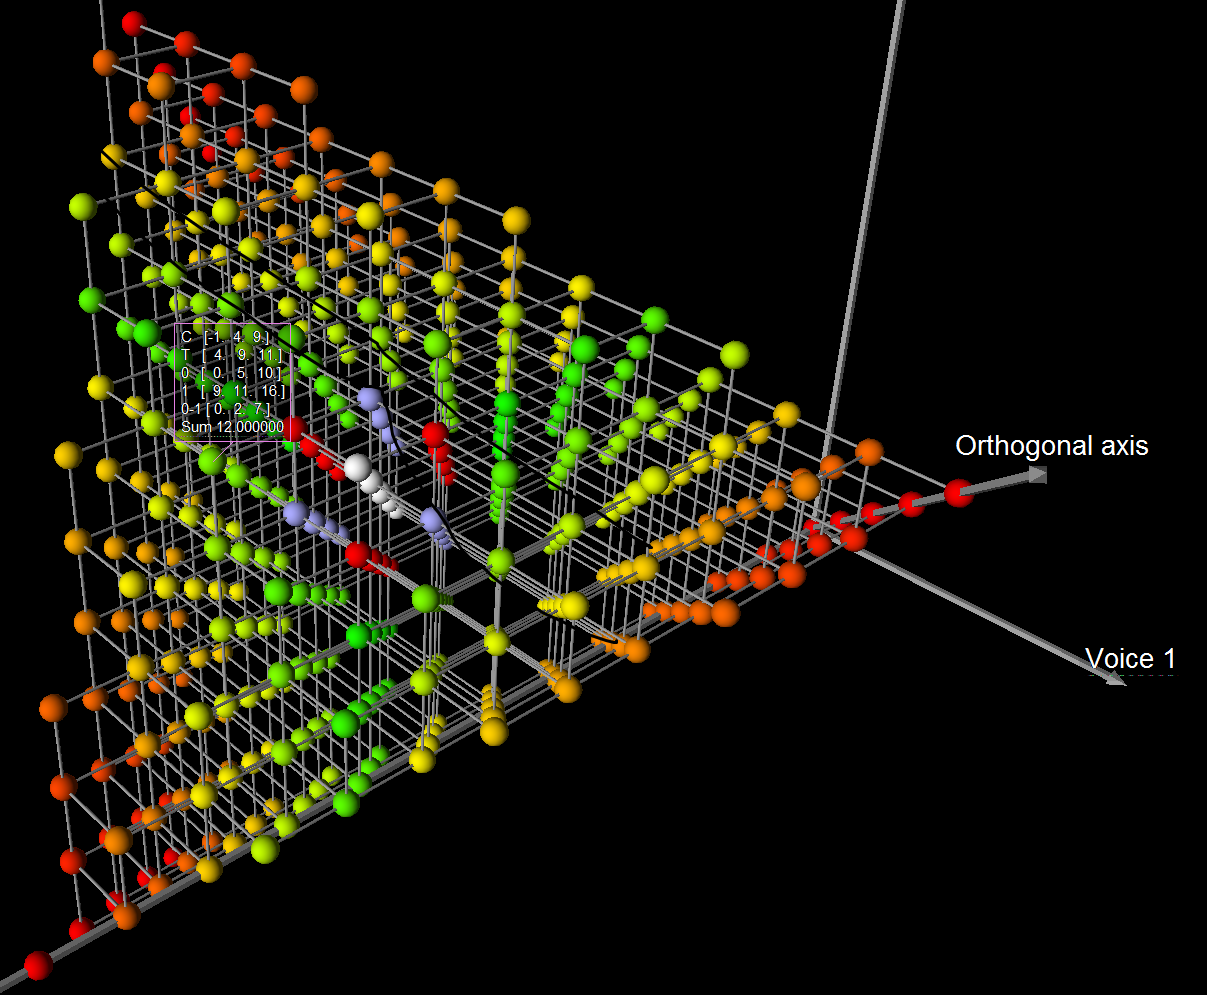
\includegraphics[width = 0.9\textwidth]{opc}}
\caption{\label{fig:opc}
  $OPC$ for trichords in 12TET.}
\end{figure}

If in addition transpositional equivalence is assumed, the orbifold collapses to
a single layer $\left(\mathbb{R}/12\mathbb{Z}\right)^{n-1}/\mathcal{S}_{n}$, in
which points at 120 degrees rotation are equivalent (Figure \ref{fig:opttc}; to
simplify the view, pitches are rounded by semitone). This is $OPTC$, which is
what musicians normally mean by ``chord type.''

\begin{figure}
\centerline{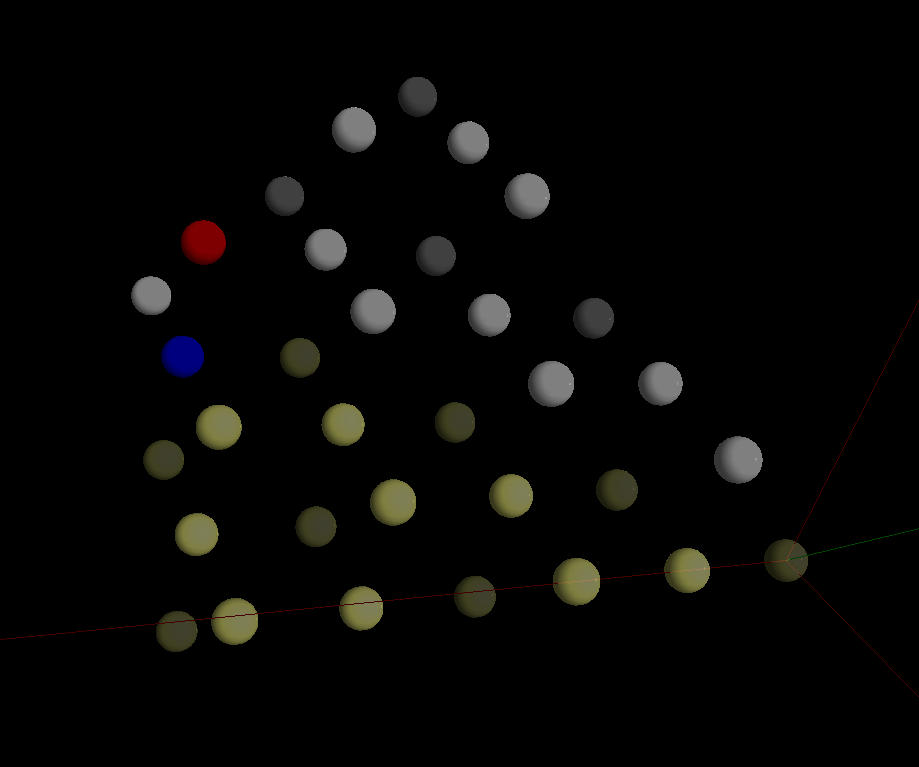
\includegraphics[width = 0.5\textwidth]{opttc}}
\caption{\label{fig:opttc}
  $OPTC$ for trichords in 12TET.}
\end{figure}

A little more theoretical sophistication reveals \textit{inversional
equivalence}: a major triad is somehow the same as a minor triad. The orbifold
folds over or reflects to equate major and minor
$\left(\mathbb{R}/12\mathbb{Z}\right)^{n-1}/(\mathcal{S}_{n} \times
\mathbb{Z}_{2})$ (Figure \ref{fig:optic}; again, rounded by semitone). This is
$OPTIC$, which is what theorists mean by ``set class,'' and is the most abstract
commonly used concept of what is a ``chord.''

\begin{figure}
\centerline{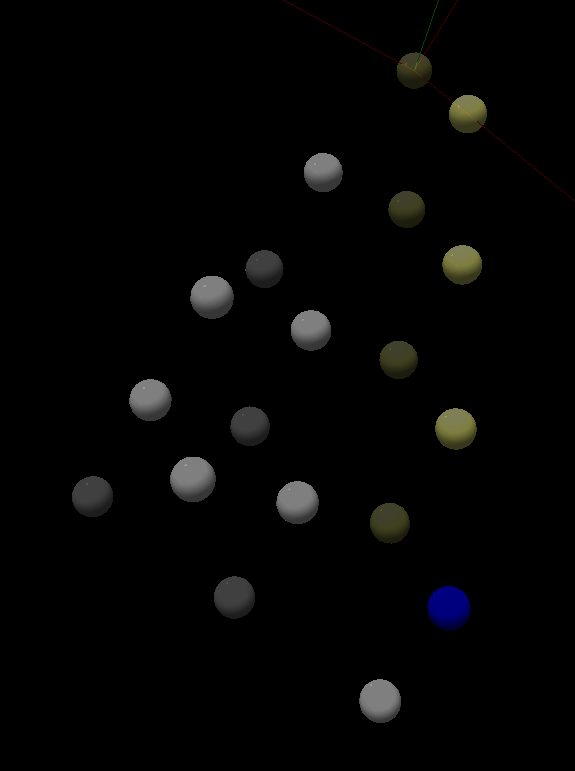
\includegraphics[width = 0.25\textwidth]{opttic}}
\caption{\label{fig:optic}
  $OPTIC$ for trichords in 12TET.}
\end{figure}

Here, we do not use chord space for composing. Rather, we construct a parameter
space in which each of the irreducible symmetries of chord space identified by
Callender, Quinn, and Tymoczko is a separate dimension, on which a specific
operation is indexed. These are:

\begin{enumerate}
\item $P$ (Callender, Quinn, and Tymoczko's $OPTIC$ space) -- Set class, the
most abstract conception of a chord; all major and minor triads are equivalent.
The number of elements in P depends upon the maximum number of voices and the
number of divisions of the octave.
\item $I$ -- Inversion.
\item $T/R$ -- Transposition within a specified range $R$.
\end{enumerate}

\noindent To these we add:

\begin{enumerate}[resume]
\item $v$ -- octavewise revoicing (within some specified range) of the $PIT$
chord, through all permutations of the possible voicings.
\item $a$ -- Voicewise re-arrangement of voices or instrument, through all
permutations of the possible arrangements.
\end{enumerate}

\noindent Obviously not all dimensions of this odd parameter space are
continuous. The purpose of $PITva$ space is to permit composing by moving a
single point through the space and thus controlling at once set class,
inversion, transposition, voicing, and arrangement; another way of saying this
is that any piece of note-based music can be represented by the graph of a
vector-valued function of time,

$$(P, I, T, v, a) = r(t).$$

By assigning each symmetry to an orthogonal dimension of the $PITva$ space, the
IFSs to be developed for composing are guaranteed to control the dimensions
independently, \textit{e.g.}\ to generate arpeggiations without affecting
chord type.

\subsection{Fractal Approximation}

A \textit{fractal} is simply a set of points that fills some definite fraction
of its space. A line on the plane occupies no space. A snowflake curve
iterates bending segments of its sides to infinity, and thus comes to occupy
some fraction of the plane (Figure \ref{fig:kochflake}
\cite{Mandelbrot:1982:FGN}).

\begin{figure}
\centerline{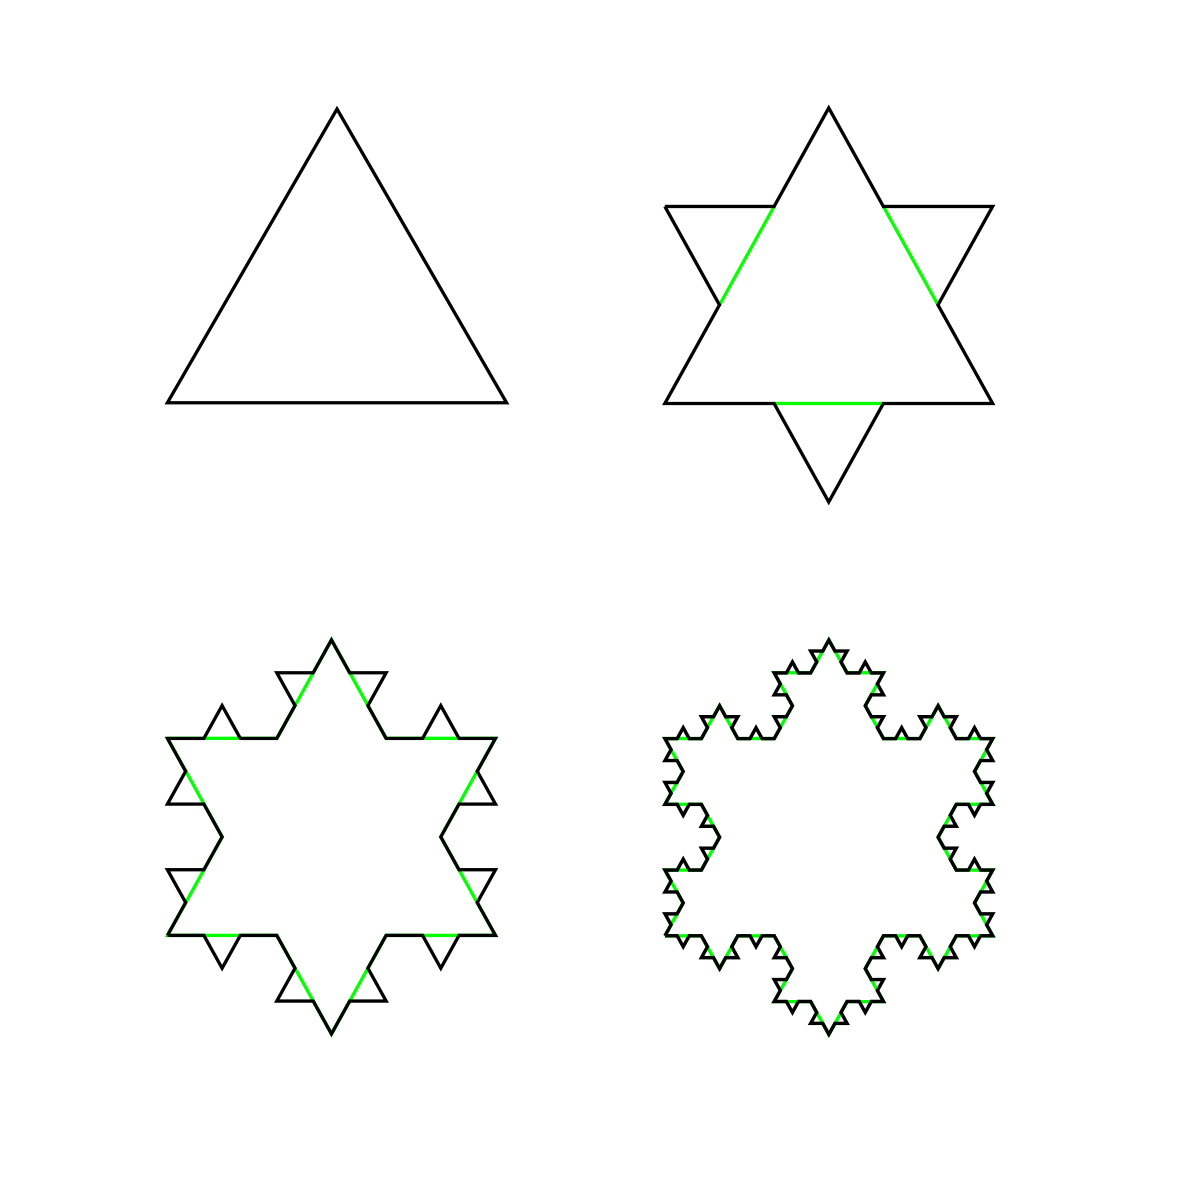
\includegraphics[width = 0.6667\textwidth]{KochFlake}}
\caption{\label{fig:kochflake} Koch snowflake
curve.\protect\footnotemark}
\end{figure}

\footnotetext{Image in \ref{fig:kochflake} licensed Creative
Commons Attribution-ShareAlike 3.0 Unported.}

One basic way to generate fractals is with the multiple copy reduction
machine (MCRM). Imagine a copier with more than one lens, each equipped with
adjustments (sliding, shrinking, or rotating the image of the original). Make
a copy, replace the original with the copy, and repeat to infinity. Just as
with the snowflake curve, the final copy comes to occupy a definite fraction
of the picture plane and thus is a fractal \cite{chaosandfractals}.

Mathematically, the MCRM is an iterated function system (IFS). Each lens
represents an affine transformation of the plane. Each lens, chosen at random
or in turns, transforms the original set, and the union of the transformations
replaces the original. More formally, an \emph{iterated function system (IFS)}
is a topological space $\mathbb{X}$ with a finite set of continuous functions
$f_{n}:\X\rightarrow \X$,
$n=1,2,\dots,N$. If the functions or transformations are contractive, the
Banach Fixed Point Theorem proves that iterating this process to infinity
brings the original to a fixed point, the attractor of the IFS
\cite{chaosandfractals, barnsley1985iterated, 10.2307/24893080,
fractalseverywhere}. An \emph{attractor} of the IFS $\cal{F}$ is a set
$A\in \cal{H}(\X)$ the set of all closed compact subsets of $\X$ such that

\begin{enumerate}
\item $\cF(A)=A$, and
\item there is an open set $U\subset \X$ such that $A\subset U$ and
$\lim_{k\rightarrow\infty}\mathcal{F}^{k}(S)=A,$ for all $S\in \cal{H}$ with
$S\subset U$; the limit is with respect to the Hausdorff metric on $\cal{H}$.
\end{enumerate}

\noindent Thus, \textit{any} original will end up producing the
\textit{same} attractor.

Furthermore, Barnsley's Collage Theorem \cite{barnsley:1986:solution} proves
that any original set can be approximated, as closely as desired, by some IFS.

This is done by arranging the affine transformations to cover the original set
with transformed copies of itself, minimizing overlaps. Let
$(\mathbb{X},d_\mathbb{X})$ be a complete metric space. $(\calH (\X),
d_\calH)$
is the associated metric space based on the hyperspace of nonempty compact
subsets of $\X$ with Hausdorff metric $d_\calH$. Assume $M\in\calH(\X)$ and
$\varepsilon > 0$. Assume $\cF := \{\X; f_1, \ldots, f_N\}$ is a contractive
IFS such that

\be\label{hutchop}
d_\calH \left(M, \;\bigcup_{i=1}^N f_i (M) \right) < \varepsilon.
\ee

\noindent Then

\[
d_\calH (M, A) < \frac{\varepsilon}{1-s},
\]

\noindent where $A$ is the attractor of the IFS and  and $s :=
\max\{\mathrm{Lip}\,f_i\st
i = 1, \ldots, N\}$.

\textit{The Collage Theorem is the key motivation for using IFSs in
algorithmic music composition}. The theorem proves that IFSs, while
conceptually simple, are as musically powerful as one might like.

The remainder of this paper concerns how to control this power: how to
filter out as many of the musically useless productions, which of course are
overwhelmingly more numerous, as possible; and how to explore the
remaining vast parameter space of IFSs in a \textit{musical} way.

It would be possible to use IFS to generate sound grains on a grid; to
generate notes on a grid; or to generate a path through a different chord
space, \textit{e.g.} use Callender, Quinn, and Tymoczko's OPC $\times$
revoicings $\times$ rearrangements instead of $PITva$. Again, our purpose is
to filter out unmusical productions. Since by the Collage Theorem IFSs are
universal, we cannot exclude such productions; but we \textit{can} simply make
it harder, take more steps, to generate then. This is not an esthetic
judgement. We are simply trying to make the score space more like the
geometry, as implied by music theory, of human musical perception.

So, we have a piece as a sequence of points in $PITva$ space, \textit{i.e.},
the graph of a function of time in that space. Graphs of functions,
\textit{i.e.} fractal approximations, can be computed by a special kind of IFS
associated with a \textit{Read-Bajraktarevi\'c} operator $\Phi$. Suppose we
are given a finite family $\{l_n : X\to X \mid n = 1, \ldots, N\}$ of
injective contractions with the following two properties:

\begin{align}
&X = \bigcup_{n=1}^N l_n(X);\label{union}\\
&\Int (l_m(X))\cap \Int(l_n(X)) = \emptyset, \quad\forall\;m, n\in \{1,\ldots,
N\}, m\neq n.\label{partition}
\end{align}

\noindent Here, $\Int (S)$ denotes the interior of a set $S$.

Suppose that $(Y,d_Y)$ is a complete metric space with metric $d_Y$. A mapping
$g:X\to Y$ is called \emph{bounded} (with respect to the metric $d_Y$) if
there exists an $M> 0$ so that for all $x_1, x_2\in X$, $d_Y(g(x_1),g(x_2)) <
M$. Then the Read-Bajraktarevi\'c operator is defined as

\be\label{RB}
\Phi g (x) := \sum\limits_{n=1}^N F_n (l_n^{-1} (x), g\circ l_n^{-1}
(x))\,\chi_{l_n(X)}(x),
\ee

\noindent where $\chi_M$ denotes the characteristic function of a set $M$.
Equivalently, \eqref{RB} can also be written in the form

\be\label{3.3}
(\Phi g \circ l_n) (x) := F_n (x, g(x)),\quad x\in X, \;n = 1, \ldots, N.
\ee

%\noindent The operator $\Phi$ is well-defined and since $g$ is bounded and each
%$v_i$ contractive in the second variable, $\Phi g\in B(X,Y)$.

This obviously is an application of the Collage Theorem. Each mapping is
actually a bilinear transformation (in the computer graphics sense, not the
digital signal processing sense) that is rescaled to fit within the
interpolation points (Figure \ref{fig:fif}).

\begin{figure}
\centerline{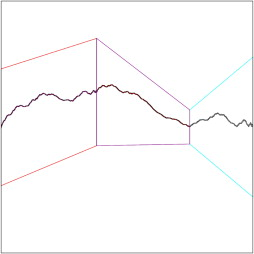
\includegraphics[width = 0.5\textwidth]{interp}}
\caption{\label{fig:fif} Three bilinear transformations in
a fractal interpolation function.\protect\footnotemark}
\end{figure}

\footnotetext{Image in \ref{fig:fif} from \cite{barnsley2015bilinear}.}

However, the flexibility of FAs can be increased by using a
\textit{local iterated function system}. A local IFS is one in which the
transformations in the IFS have the same co-domain, but not necessarily the
same domain. The individual domains must not overlap.

The association of the RB operator $\Phi$ with the IFS of a score graph $G(r)$ is
shown in this commutation diagram:

\be
\begin{CD}
X\times Y @>\cF_\Phi>> X\times X\\
@AAGA                  @AAGA\\
B(X,Y) @>\Phi>>  B(X,Y)
\end{CD}
\ee

\noindent where $G$ is the mapping $B(X,Y)\ni g\longmapsto G(g) = \{(x, g(x))\mid x\in X\}\in X\times Y$.

Please note, and do not forget, that here we use the \textit{graph} of a bounded
fractal function to represent a musical score, not the fractal function as such.
Our purpose in using the RB operator is to ensure that we generate \textit{only} IFS
that compute score graphs.

The IFS that computes the graph of the fractal function can be expressed:

Next, we exhibit the relation between the graph $G$ of the fixed point $f^*$ of the operator $\Phi$ given by \eqref{RB} and the local attractor of an associated contractive local IFS. To this end, we need to require that $\X$ is a closed subset of a complete metric space. Consider the complete metric space $\X\times\Y$ and define mappings $w_i:\X_i\times\Y\to\X\times\Y$ by
\[
w_i (x, y) := (u_i (x), v_i (x,y)), \quad i\in \N_N.
\]

In this equation, the $u$ functions transform the graph in the direction of the
\emph{domain} $t$ of the graph, and the $v$ functions transform the graph in the
direction of the \emph{range} of the graph.

The family $\cW_\loc := \{\X\times\Y; (\X_i\times\Y, w_i)\st i\in \N_N\}$ is a contractive local IFS in the metric $d_\theta$ and the graph $G(f^*)$ of the local fractal function $f^*$ associated with the operator $\Phi$ given by \eqref{Phi} is an attractor of $\cW_\loc$. Moreover,
\be\label{GW}
G(\Phi f^*) = \cW_\loc (G(f^*)),
\ee
where $\cW_\loc$ denotes the set-valued operator \eqref{hutchop} associated with the local IFS $\cW_\loc$.


\subsection{Hilbert Indices for Fractal Approximation Parameters}

\section{Implementation Notes}

See https://www.marksmath.org/scholarship/ReadBajPP.pdf.

Any Hutchinson operator is an RB operator if its member affine transformations do not have overlapping domains.
Many methods can be used to ensure this. Here, we adapt an algorithm that has been used to recursively compute
Koch curves. A recursive function takes a list of bilinear transformations, a parent domain, a container for
iterated points, and a limit of iteration (which can be an actual count of iterations, or a quantization interval).

The contractions of the domain in each bilinear transformation are not given directly, but as a fraction of the
parent domain. The translations of the domain in each bilinear transformation likewise are not given directly,
but have added to them the implicit translation

\section{Musical Examples}

\subsection{Parametric Mapping}


\subsection{Interpolating Between Pieces}


\subsection{Using the Genetic Algorithm with Fractal Interpolation
Functions}

\section{Future Directions}

It is interesting that, as Massopust notes \cite{massopust2017},
\begin{quote}D. Hardin proved in 2012 that every compactly supported
refinable function is a piecewise fractal function. In particular, the
unique
compactly supported continuous function determined by the mask of a
convergent
subdivision scheme is a piecewise fractal function. \end{quote}
This implies that the same technique of parametric
composition based on FAs and described here, would also work for composing
sound directly using refinable sets of sound grains, \textit{e.g.}
wavelets.

It also is interesting that Barnsley, Hegland, and Massopust
\cite{2013arXiv1309.0972B} discuss how to derive fractal approximations of
existing data sets. This implies that it is possible to automatically
derive
FA parameters for existing works of note-based music, and then to use the
resulting parameter map or parametric interpolation to analyze the
relationship between the works, or to compose new works intermediate in
form
between them.

\section{Correspondence between Recursive Koch Constructions and Fractal Functions}

I used to make pieces using Koch constructions, either nested for loops, or recursive
functions proceeding to a predefined depth.

It occurs to me that the recursive Koch construction (RKC) may be equivalent to a
fractal function (FF) based on an IFS, and may even lend itself to the implementation
of fractels.

In the RKC, the transformations are guaranteed to exactly divide the range of the
function at each stage of iteration, and to be applied exactly and only within the
parent division. In the RKC, as in the FF, the transformations include no rotations and
produce no overlaps between segments (iterations).

It is not necessary to iterate the RKC to infinity, and indeed it is not necessary to
iterate the RKC below the scale of the semitone.

Both the RKC and the FF when iterated to infinity have a fixed point if the systems are
contractive.

Fractels can be implemented by selecting transformations based on the value at the domain.

The algorithm can proceed to just below the scale of the semitone. The produced points
(notes) can then be quantized and overlapping notes joined.

How can I prove the equivalence between RKCs and FFs? I will try to do that.

\printbibliography
\end{document}
